\section{Toward a Corpora of Cinematic Interactive Narrative Player Experiences}
\label{sec:orgheadline1}
Narratives are a fundamental mode of discourse, and a topic of intense
interest in the AI community since the beginning. The form represents
a sophisticated communication of not only information about a
particular series of events, but various perspectives on them that are
encoded in the telling. Storytellers rely on these methods to achieve
various effects, and often psychology and social sciences rely on
narrative context to conduct experiments due to the strength that a
narrative understanding exerts over emotional response and perception
of new events.

This paper describes an exploratory, corpus-based approach to conducting interactive narrative research in order to address several issues with current approaches. First, current work is often, due to cost and practical reasons, conducted on works created by researchers for the purpose of research. While many of these serve as a viable testbed for isolating particular narrative effects, they do not represent the current state of interactive narrative in the entertainment industry. Many story-based games that are popular today are backed by large budgets and include mimetic storytelling over text-based storytelling. As a result, these experiences closer resemble cinema than literature, and the production quality of the final work is simply out of the reach of research labs budgets. Second, there are no current accepted methods or approaches to comparing competing models of narrative on equal footing. A major contributor to this is the lack of availability of datasets which allow for comparing models. Third, the tools that we have for discerning and measuring effects of narrative are improving, but they require additional work to assemble a study to validate. This suggests that a shared resource of data, content and raw results which is not designed for a particular study would be of general use, as has been the case in the computational linguistics community. 

To this end, we propose a corpus-based approach to studying interactive narrative that focuses on long-form, released episodic games and which leverages as much data collection as possible for the testing and refuting of models and theories. We have begun this work by recording a set of player experiences of the contemporary interactive fiction piece “The Wolf Among Us” by Telltale Games, and have analyzed the initial set of annotations with the goal of finding patterns in emotional reports by players.

This paper is organized as follows: First, we motivate the current work by arguing for the study of long-form episodic interactive narratives and further characterize the sub-genre of choice-based cinematic adventure games (CCAG) as a primary avenue for focus. Second, we review the existing methodologies and research approaches that have used computational means to study both static and interactive narrative, and pay particular attention to those that include measurement and characterization of the player experience and emotions. We then describe the study design and initial annotations applied to the dataset. Finally, we describe the results of comparing the usage of the instrument with the annotated choices of the participants and observe that the hypothesized clustering of usage around significant decisions or events was not present. We close with a discussion of future research to be done based on availability of a corpus of interactive fiction playthroughs.
\section{Motivation}
\label{sec:orgheadline2}
Narrative media accumulates meaning over time; a given event can color future events while a given detail properly foreshadowed can complete a final plot flourish.A work’s effect results from the totality of material, resulting in an impression of a world and its inhabitants. Many of the effects of a particular representation of media are also additive: the linguistic meaning of a particular dialogue exchange may be undercut by the treatment in the language of cinematography.

The holistic nature of many modern commercial interactive narratives raises many research questions about interactions between story and interaction choices, presentation modes \cite{Springel1998-gm}, or game mechanics \cite{Larsen2016-sk}. The proposed approach of using a corpus of real player traversals is not an exhaustive analysis of the potential experiences present in the artifact itself, as such would require investigating every possible combination of choices. Instead, by using a set of player experiences of the interactive narrative we can understand the range and types of reactions to the artifact as well as the specific affordances in the genre that may have given rise to them. Consequently, the schema proposed in this is specific to the genre of games that Telltale has popularized, and would need to be extended as each game in the series often introduces novel interactions that heighten or deepen the narrative engagement.
\section{Related Works}
\label{sec:orgheadline11}
This project crosses many boundaries of traditional efforts, charting
both a non-textual interactive narrative as well as one that is
previously published. The following sections describe the current
efforts in both modeling narratives as well as understanding player
experiences.

\subsection{Modeling Narratives}
\label{sec:orgheadline3}
Following in the original models of meaning in artificial intelligence
research started by Shank with conceptual dependencies, a number of
approaches have been developed by the community over the years to
capture aspects of narrative in a computable model, with either the
goal of understanding the model as a human would need, or in using
these models to create a story. There are a number of efforts underway
to model narratives, including NarrativeML (Computational Narrative)
\cite{Mani2012-py}, the drama-focused ontology Drammar
\cite{Albert2016-ij,Larsen2016-sk,Rapp2001-ea}. David Elson has also
taken a computational linguistics approach to charting narrative
discourse using a semantic graph based approach. Much of his work with
Story Intention Graphs \cite{Elson2012-pi} and in particular focusing
on descriptive methods has been an inspriation to the present work. He
has made publicly available corpus of stories, the DramaBank
\cite{Elson2012-xn}. Sarah Harmon has begun revisiting the goals of
SIG with a human-readable textual management system.

\subsection{Annotating interactive media}
\label{sec:orgheadline4}
Interactive media presents novel challenges compared to the linear
media that is the focus of the descriptive models in section
2.1. There have been many efforts to operationalize these models of
narrative to create novel storytelling systems, but relatively few
efforts to document and analyze existing interactive narratives of
which source code is unavailable. One of the first roles of the
Hypermedia model was to provide a specification of what that name and
product could look like with a focus on static content and linear
media connected via annotations \cite{Hardman1994-xs}. In a more
descriptive vein, the OntoMedia project \cite{Jewell2005-ya} seeks to
identify parallel content in and amongst heterogeneous media. One type
of result that came from the model was the evaluation of prominence of
a character in a work in a written version versus a film adaptation..

\subsection{Choice-Based Interactive Narratives}
\label{sec:orgheadline5}
One of the primary features of the choice-based cinematic adventure game is the emphasis placed on the moment-to-moment timed choices of the player over puzzle solving, combat or other interactions. While combat and other tense events are often represented by “quick-time events,” the majority of the content is delivered by dialogue among a set of characters acting out essentially an interactive script. The gameplay is evocative of cinematic works, showing a changing perspective between characters and also incorporating shot types often seen in film and television and not often present in the middle of a typical roleplaying game. Fendt et al investigate the role of actual agency versus perceived agency in text-based games. Their study compared actual branching storylines with those that are similar to the structure of Telltale games, which includes primarily short-term feedback of the responses to a particular choice \cite{Fendt2012-xe}

Peter Mawhorter has made contributions to understanding choice
poetics, synthesizing a range of research into a foundation for a
theory of choice aesthetics \cite{Mawhorter2016-cx}. In it, Peter not
only devises a set of narrative dimensions to map his work across, but
also assesses the measures he developed through an online gam. The
main shortcoming of his approach, analyzing choices based on player
goals, is the diverging set of player goals and identities vital to
the work itself. Cardona-Rivera et al take a different approach with
their analysis of choices, using a situation model to decide whether
choices were in fact meaningful or not based on whether a choice would
result in a change in the situation is some way
\cite{Cardona-Rivera2014-ed}. Both studies have focused on textual
choose-your-own-adventure style games and thus miss out on the
opportunity to see choices influenced by non-textual factors such as
tonality, dramatic presentation, cinematographic or even visual
appearances. Many subtle influences are exerted in The Wolf Among Us
either by the characters themselves or by the creators to influence a
particular interpretation of events or characters, and the choices
often feature and reinforce that interpretation heavily.  
\subsection{Player and Player Experience Modeling}
\label{sec:orgheadline6}

Many works have started charting the specific reactions of players to
interactive narratives. The exact nature of how reader response is
shaped is theorized by Mani \cite{Mani2010-sh}, whose focus is on the
evaluation of characters by the reader, whereas along a similar vein
but Battaglino and Damiano focus on the character appraisal of each
other \cite{Battaglino2014-gh}. Part of the tendency is to model these
effects with a goal of optimization, or finding an ideal model to
represent the reader’s response or the character’s affect. In contrast
to this, Roque engages directly with the hermeneutics of literary
complexity in text \cite{Roque2012-fd}, a reminder that the sheer
amount of meaning embedded in a communicative media may not be
amenable to reductive approaches, again with a focus on uncovering the
meaning of existing works rather than generating them themselves.

Some of the more successful approaches to using planning and knowledge
of the storyworld to create or understand specific effects include
suspense \cite{Cheong2007-ts}, surprise \cite{Bae2008-js}, tension
\cite{Szilas_undated-am}, interestingness and specific emotional
responses \cite{Roberts2009-km,Hernandez2014-hd}.  Part of the desire
to understand the interactions and the totality of a longer, fully
produced work is what motivates the current approach.

Another strain of work has focused on the communicated experience of
expressive characters within drama, in particular their
emotions. Annotating Character Emotions in Drama
\cite{Damiano_undated-sx}

Katherine Isbister et al developed the Sensory Evaluation Instrument
\cite{Isbister2006-sc,Laaksolahti2009-uw}. While we are not using
every aspect of the SEI in the present study, its use is tabulated to
evaluate basic affective response and the video is saved along with
the annotations for future use.
\subsection{Goals and Requirements}
\label{sec:orgheadline7}
Given the current efforts in studying narratives and in particular
experiences of players and interactive narratives, we assembled a set
of requirements for a player experience corpus that would application
of existing methods and models as well as facilitate experimentation
with new methods and approaches. Because we wanted to establish
methods that could both be used for different purposes and for future
approaches to compare against current approaches, we tended to err
toward a more holistic documentation of the experience from as many
measurable and nonmeasurable records as possible. Nevertheless, the
following requirements stood out:

Synchronizing annotations of player observation and gameplay
footage. This enables training of machine learning algorithms to
eventually automate any of the tagging that may take place or be used.
Annotating specific events in the playthrough. This includes any event
that can be identified through a videofeed of the gameplay itself or
by the player’s interaction with it.  Connecting events across
“shared” content. An audience watching a movie all witnesses the same
story. In the case of interactive stories, the prior events or even
the selected response of the player-character may vary significantly,
and these lead to potential problems when comparing a player’s
response to the same content. The method should allow for tracking
both current content choices as well as prior choices that led up to
it.  Enable future elements derived from the gameplay footage,
e.g. gaze, expression, posture to be visible and able to be connected
to the other annotated features
\subsection{Telltale Games’ \emph{The Wolf Among Us}}
\label{sec:orgheadline8}
With these goals and requirements in mind, we selected Telltale Games’
The Wolf Among Us as it had an acceptable amount of complexity and
narrative variation while taking advantage of many of the
emotional-targeting authoring techniques often used for modern
televisions). In this section we’ll review the overall game, including
plot for the first episode, as well as the types of dramatic scenarios
present.

Telltale Games has similar goals to television series creators, that
of emotional storytelling. As a result of its original has defined
this genre with

By working with a popular game genre, we can apply computational
methods to the communities of discourse surrounding it. Many players
discuss their choices and their experiences either through
self-published videos of their own playthroughs, or through discussion
forums.

First, the plot focuses on an investigation by the player-character
protagonist, Bigby Wolf, of a murder in the community of Fabletown,
where creatures and characters from bedtime stories have been forced
to flee their homelands and take up residence in New York City. The
game is based on a comic series by Bill Willingham, and has been since
adapted into a canon issue ahead of time.

An important thematic and core draw for the story is the portrayal of
a poignant class divide within the currently causing friction between
the non-human Fables, such as the first character introduced,
Mr. Toad, and the human fables. Not only are the non-human Fables
unable to live in the desirable luxury apartment complex, where the
mayor’s office and sheriff are, but they are mandated to wear a
special enchanted item called a Glamour that gives them any appearance
possible.

The game is divided into 6 chapters, with the 4th chapter being
essentially a choice of ordering of two scenes within the 5th chapter
(having Snow and Bigby visit either Toad’s apartment or Prince
Lawrence’s apartment first). The game primarily employs choices in the
form of timed sets of buttons to respond to a particular situation as
the player-character. Often the player-character will also deliver
lines and actions without prompting to either set up the scene or
deliver a necessary kernel for each story. While analyzing the game
for the pilot study, a number of types of mechanics were identified by
their functionality. The three primary ones are dramatic choices,
exploratory choices, and game choices. The focus of the present study
is on dramatic choices, which are characterized by values and
relationships over material gain or access.
\subsection{Study Design}
\label{sec:orgheadline9}

We conducted a preliminary study with 7 participants. Each participant was instructed to play through the first episode of The Wolf Among Us, using All the Feels (ATF) \cite{Robinson2016-qr}, Sensual Evaluation Instruments (SEI) \cite{Laaksolahti2009-uw,Isbister2006-sc}, and think-aloud techniques. Post game, the participant did a retrospective think aloud and filled out the Immersive Experience Questionnaire (IEQ). We wanted to know the benefits of this emotion evaluation suite at various points of play. As a prerequisite to participate in the study, we required that the participant had never played the game before so their reactions would be unadulterated. We chose this particular game because of its easy controls to pick up for a non-gamer, as well as its range of narrative mechanics and emotional palette. The work represents a subgenre of adventure game that focuses on moment-to-moment player choices relating to dramatic beat \cite{Murray2017-ak} As why we chose it]
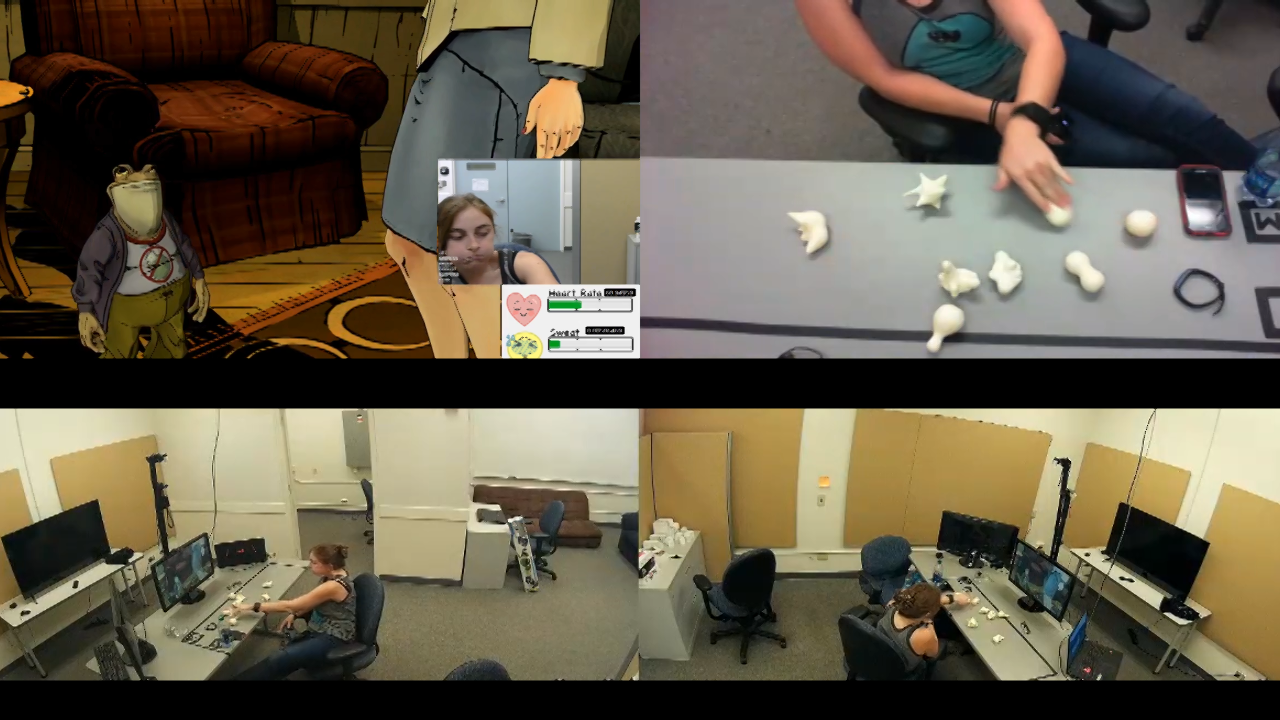
\includegraphics[width=.9\linewidth]{Player6ReactionSynced.png}
At the beginning of the session, we started by having players take a
pre-game questionnaire, asking them a variety of questions relating to
familiarity with the Fables comics lore the game is based off of or
any other telltale games which may bias their feelings. We then
calibrated the SEI, which consists of showing the users a set of 10
photos of different images and having them indicate with the SEI which
association came to their mind for that particular instrument.  We
then instructed participants to play the game, think aloud, as well as
use the SEI as much as possible. They were also equipped with the
Empatica E4 wristband (ATF) to track their HR and GSR data. The facial
recognition, Affdex, from ATF was running as well
\cite{Robinson2016-qr} At the end of the session, we conducted a
retrospective think-aloud with the player about how they felt at
certain peak moments of the game, how they felt about various
characters, and why they used specific SEI during play. We then
instructed them to take the IEQ as an additional method for
comparison. We then analyzed the data and correlated the
moment-to-moment choices with use of the SEI, biometrics, and
think-aloud.

We needed to annotate the actions taken during the playthrough, the
presented choices, and any player reports of emotions. Cinematic
choice-based adventure games employ a variety of interaction
mechanics. These include inventory (keeping track of items that affect
choice availability), navigation (moving through a 3D environment
which displays “hotspots” indicating possible interactions. These can
also affect the state of items in the environment, such as whether a
fan is on or off, and include triggering “satellite” content such as
the player-character commenting on a particular item in their
apartment (see \cite{Chatman1980-rl}). We understand that modeling the
full diverse range of mechanics does not need to be done all at once,
and so we focused on the aspects of the game most apparently tied to
emotional states of players.

We focused on a subset of features were the simplest to identify by
visual inspection without resorting to inter-annotator agreement
validation. These included the timecode and set of alternatives of
each choice presented to the player and the ultimate player decision
(including not making a choice in time). The timing and the content
are used to further analyze the player’s emotional context after such
choices by comparing the timecodes of the instruments to that of the
choices. We began the annotation process by making use of a research
tool designed for multi-modal annotation of videos, Anvil
\cite{Bunt_undated-ey}, an openly available video annotation tool for
annotating playthrough data. Anvil represents annotations on “tracks”
which allows for a set of annotations that have attributes with
various types associated with them. We eventually completed the
annotation using the marker feature of Adobe Premier Pro due to the
sheer amount of footage, totaling at over 13 hours. The main advantage
of Premier Pro over Anvil was the ease with which speed could be
controlled, although specifying ranges for annotations was not as
easily done. We exported the annotations into a CSV format for further
work, which consisted of identifying the choice point and transcribing
the choices text.

We decided to start exlporing the dataset by charting the extent and
variance of this new dataset, and so proceeded with mostly objective
and easily annotated features without the need for inter-annotator
agreement to validate the annotations. The next section presents and
discusses the initial metrics of the playthroughs.
\subsection{Initial Results}
\label{sec:orgheadline10}
While we aimed to collect as comprehensive a set of measurements on
the actual player performance and expressions during the traversals as
possible, we report our early analysis on the metrics that were easily
annotated.

\begin{center}
\begin{tabular}{rrrrrrrrrrr}
Player & Duration & SEI Uses & Doubleball & Ball & Spiky & Bubbly & Pseudopod & Barba papa & Anteater & Stone\\
\hline
1 & 1:51:55 & 8 & 2 & 1 & 2 & 2 & 1 & 0 & 0 & 0\\
2 & 1:42:05 & 14 & 3 & 1 & 3 & 0 & 2 & 2 & 2 & 1\\
3 & 2:01:46 & 30 & 2 & 0 & 4 & 3 & 8 & 1 & 9 & 3\\
4 & 1:55:39 & 70 & 12 & 3 & 8 & 11 & 12 & 4 & 14 & 6\\
5 & 1:44:25 & 49 & 2 & 1 & 2 & 12 & 13 & 6 & 11 & 2\\
6 & 1:53:30 & 82 & 12 & 3 & 7 & 19 & 13 & 9 & 12 & 7\\
7 & 1:54:07 & 14 & 3 & 1 & 4 & 1 & 1 & 1 & 3 & 0\\
\end{tabular}
\end{center}
In order to correlate the decisions among players, a coding schema was
devised that incremented a scene number whenever a change in character
occurred, and which incremented a choice set number each time an
interface was presented. This enabled some amount of flexibility in
identifiers to agree when certain choice paths led to additional
choices, as was the case several times. There were two game segments
that included non-dramatic gameplay mechanics. The first was the
office, where the player gradually learned that the identitiy of the
prostitute was a Fable named Faith. While this segment was vital for
backstory, the mechanics are largely that of hypertext. The second
divergence was during a scene with Mr. Toad where Bigby is questioning
him about suspicious circumstances. In this scene the exploratory
mechanic supports a game of pointing out inconsistencies and forcing
Mr. Toad to admit why he was concealing a break in. Interestingly, the
dramatic tension in this scene is in part built up by earlier
exchanges with Mr. Toad which may provoke the player to side against
the character. One of these is an aside given by Mr. Toad when Bigby
has passed away, cursing the Sheriff for telling him “how to spend his
money”. Such a scene plays the dual role of establishing the class
theme as well as providing the player a ready-made set of
relationships to base their interpretation of the character on.

Because of the focus of this initial study on emotions and choices, we
focused exclusively on dramatically staged choices. We also recorded
variants of choices based on state variables. We decided on 25
distinct scene units, some of which occurred in different orders. Some
scenes are single choice sets, such as the final decision as to
whether to arrest Dee or the Woodsman.

We found that there were 6 choices which received unanimous agreement
in the decision from all of the participants. Three of these choice
sets were strongly influenced by the presentation of the choices
within the game. One of the choices was a final dilemma of who of the
two available suspects to arrest. Interestingly, all of the
participants chose to arrest Dee, most likely because of the revealing
scene that caused the Woodsman to confess another crime during the
final scene of the game. Another 10 questions were agreed by 6 out of
the 7 participants, including not disclosing a character’s presence,
Beauty, to her husband, Beast by lying. The vulnerability of Beauty’s
request and its primacy may play a role in its preference, much as the
first sequence is designed to elicit player’s attachment and sympathy
for Faith.

These findings suggest that narrative modeling will be necessary to
understand the reported diversity of player experiences.

Szilas proposed a number of measures for choice analytics
\cite{Szilas2014-fd} which we quickly realized would not apply well to
CCBA as the diversity of choices was extremely limited, with with 74
choices identically presented to all 7 participants.

\begin{table}[htb]
\caption{Annotator agreement of use of SEI on sections}
\centering
\begin{tabular}{rrl}
ID & Participants & Description\\
\hline
12-1 & 3 & Snow gets Bigby and brings him to see Faith's decapitated head.\\
15-1 & 2 & Exploring the office in the Woodlands and interacting with the mirror finding Faith's identity\\
6-1 & 2 & Visiting Prince Laurence's House and discovering he'd been shot (or shot himself)\\
\end{tabular}
\end{table}

One of the more surprising results was that only three segments had
multiple annotators express emotions during them. This was determined
by selecting SEI events by their timecode using the timecode of a
decision point and the following, or the end of the work if it was the
last. By this measure, two choice sets stood out as they were
surrounded by large spans of time. See Table 3.
\section{Future Work}
\label{sec:orgheadline12}
With an increase in the density of the data, visualization will become
ever more important. While we subjected the dataset to basic
mathematical analysis, more advanced questions relating causes from
narrative origins to potential effects will require an interactive
visual interface. Further analyze emotional data based on calibrations
and compare to other measures of emotion (for both characters and for
the player).

We would like to attempt to automate many of the more mechanical
feature detection tasks and focus annotation efforts on semantic
challenges such as meaning and story structure. To this end, we’d like
to use multiple story models on the same corpus for comparison (SIG +
Drammar, for instance).

Analyze choice paths based on the values expressed by the player both
about morals and about particular characters and visualize how they
change over time. This is well supported by this dataset.
\section{Conclusion}
\label{sec:orgheadline13}
In this paper we presented a methodology for collecting the videos of
both player behavior and gameplay captures as well as emotional and
physiological signals. We argued for the focus on longer form
commercially available works as subjects of experiments and presented
the initial results of an analysis of a study of 7 participants
playing Telltale Games The Wolf Among Us. We evaluated the
effectiveness of our corpus by comparing the usage of emotional
instruments to the choice points across a variety of traversals,
finding that the diversity in expression was not easily uncovered. We
believe there are a number of opportunities for developing holistic
models that capture narrative, emotion and context in order to
understanding player experiences in interactive narratives.
